
\makeatletter
\tikzoption{canvas is plane}[]{\@setOxy#1}
\def\@setOxy O(#1,#2,#3)x(#4,#5,#6)y(#7,#8,#9)%
  {\def\tikz@plane@origin{\pgfpointxyz{#1}{#2}{#3}}%
   \def\tikz@plane@x{\pgfpointxyz{#4}{#5}{#6}}%
   \def\tikz@plane@y{\pgfpointxyz{#7}{#8}{#9}}%
   \tikz@canvas@is@plane
  }
\makeatother 
%\resizebox{4.5cm}{!}{
% \begin{tikzpicture}[y={(-1cm,0.5cm)},x={(1cm,0.5cm)}, z={(0cm,1cm)}]
\begin{tikzpicture}[y={(-1cm,0.5cm)},x={(1cm,0.5cm)}, z={(0cm,1cm)}]
\coordinate (A) at (0,0,0);
\coordinate (B) at (2,0,0);
\coordinate (C) at (1.1*1.8,1.1*1.5,0);
%1.8/2.34,2+1.5/2.34,0
\draw[fill={rgb:red,1;white,5}] (0,0,0) -- (2,0,0) -- (2,2,0) -- (0,2,0) -- cycle;
\draw[fill={rgb:blue,1;white,5}, opacity=0.5] (0,0,0) -- (1.1*1.8,1.1*1.5,0) -- (1.1*1.8,2+1.1*1.5,0) -- (0,2,0) -- cycle;
%\node[transform shape] at (0,0) (ImageA)  {\includegraphics[width=3cm]{fig/signal_reconstruction_principle_2.pdf}};

%\node[canvas is plane={O(0,0,0)x(2.2/2.41,1/2.41,0)y(2.2/2.41,3/2.41,0)}] at (1.1,1.1) {\includegraphics[width=4cm]{fig/signal_reconstruction_principle_2.pdf}};
\node[canvas is plane={O(0,2,0)x(0,1,0)y(1,2,0)}] at (0.9,-0.9) {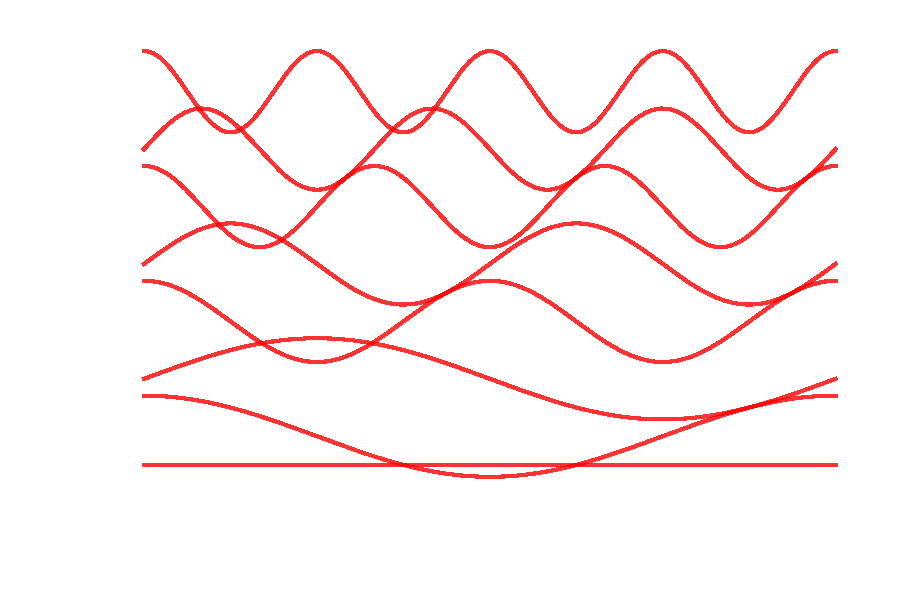
\includegraphics[width=2.4cm, height=2.4cm]{img/neurips/principalangles/signal_eigreconstruction_modes.pdf}};

\node[canvas is plane={O(0,2,0)x(0,1,0)y(1.8/2.34,2+1.5/2.34,0)}] at (0.65,-0.35,0.1) {\includegraphics[width=2.4cm, height=2.7cm]{img/neurips/principalangles/signal_reconstruction_principle_2.pdf}};

\begin{scope}
	\draw (0,-1.3,0) node[above left = 0.5mm] {$\theta_{N}(\mathcal{T}(\bm{x}),\mathcal{E}_{N}^{\mathcal{F}})$};
	\draw (2.2,-0.8,0) node[below ] {$\mathcal{E}_{N}^{\mathcal{F}} = \Span (e_{j}^{\mathcal{F}})_{j \in [N]}$};
	\draw (-0,6,0) node[below right=0.5mm] {$\mathcal{T}(\bm{x}) = \Span k(x_{i},.)_{i \in [N]}$};
    \clip (C) -- (A) -- (B) -- cycle;
    \draw[-] circle[at=(A),radius=4mm];
  
\end{scope}
% \begin{scope}[canvas is yz plane at x=1.25]
% \draw[fill={rgb:blue,1;white,5}] (0,0) -- (2,0) -- (2,2) -- (0,2) -- cycle;
% \end{scope}
\end{tikzpicture}

%}